\documentclass[12pt, a4paper]{article}

\usepackage{polski}
\usepackage[utf8]{inputenc}
\usepackage[T1]{fontenc}
\usepackage{graphicx, tikz, longtable, pgfplots, parskip, tabularx, multirow, multicol, array, geometry, longtable, csvsimple, enumitem}

\geometry{margin=1in}
\graphicspath{{obrazki/}}
\pgfplotsset{compat=1.18}
\setlength{\baselineskip}{10pt}

\title{Spadek swobodny}
\author{Konrad Grunt}
\date{Grudzień 2022}

\begin{document}

\pagestyle{plain}

\begin{center}
    \begin{tabular}{|c|c|c|}
        \hline
        \multirow{9}{*}{
\includegraphics{logopwr.png}}
        & \multicolumn{2}{c|}{}\\
        & \multicolumn{2}{c|}{\textbf{SPADEK SWOBODNY}}\\
        & \multicolumn{2}{c|}{}\\
        \cline{2-3}
        & & \\
        & \multicolumn{1}{c|}{Konrad Grunt} & 13.12.2022\\
        & & \\
        \cline{2-3}
        & & \\
        & \multicolumn{1}{c|}{Wtorek parzysty 7:30} & 5.0\\
        & & \\
        \hline
    \end{tabular}
\end{center}

\vspace{2cm}

\section{Wprowadzenie teoretyczne}

\vspace{1cm}
Równania szybkości od czasu (1) i wysokości od czasu (2):

\begin{equation}
    v(t)=gt,
\end{equation}

gdzie:\\
\(v\) - szybkość,\\
\(g\) - wartość przyspieszenia ziemskiego,\\
\(t\) - czas od rozpoczęcia spadku.

\begin{equation}
    h(t)=h_0-\frac{1}{2}gt^2,
\end{equation}

gdzie:\\
\(h\) - wysokość, na której znajduje się ciało,\\
\(h_0\) - wysokość początkowa,\\
\(g\) - wartość przyspieszenia ziemskiego,\\
\(t\) - czas od rozpoczęcia spadku.

\vspace{1cm}
Zauważmy, że spadek swobodny to ruch jednostajnie przyspieszony (z przyspieszeniem ziemskim $g$) bez prędkości początkowej.

\newpage

\section{Przebieg eksperymentu}

Ilustracja:
\begin{figure}[h]
    \centering
    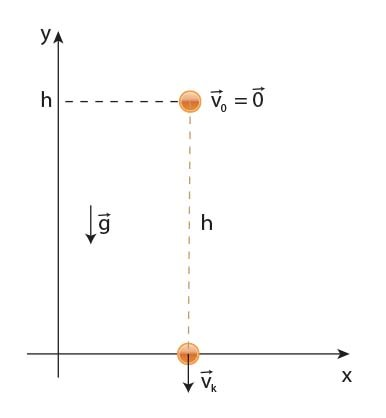
\includegraphics[width=0.5\textwidth]{obrazki/schemat.jpg}
    \caption{Schemat spadku swobodnego.}
    \label{fig:1}
\end{figure}

Jak widać na rys. \ref{fig:1}, ciało rozpoczyna spadek na wysokości $h=h_0$, bez prędkości początkowej ($v_0=0$). Porusza się ruchem jednostajnie przyspieszonym pionowo w dół (współrzędna położenia $x$ nie ulega zmianie) z przyspieszeniem $a=g=9,81 \frac{m}{s^2}$  i kończy spadek w momencie uderzenia o powierzchnię ziemi z prędkością końcową $v=v_k$.

\section{Wyniki pomiarów}

\begin{longtable}[h]{ c | c }
    \caption{Wyniki pomiarów.\label{long}}\\

    \bfseries Czas [s] & \bfseries Droga [m]\\
    \hline
    \endfirsthead
    \csvreader[head to column names]{dane1.csv}{}
    {\csvcoli & \csvcolii\\}\\
    \hline
    \multicolumn{2}{ c }{Koniec Tabeli \ref{long}}
\end{longtable}

W Tabeli \ref{long} zamieszczono wyniki kolejnych pomiarów czasu i przebytej drogi przez ciało podczas 10 sekund spadku swobodnego.

\newpage

\section{Wnioski}

\vspace{1cm}

\begin{enumerate}[label=\alph*)]
    \item Spadek swobodny to ruch odbywający się jedynie pod wpływem siły grawitacji, bez oporów ośrodka.
    \item W przypadku, gdy spadek dotyczy ciała o dużej gęstości i ma miejsce z małej wysokości w pobliżu powierzchni Ziemi, można zaniedbać opory powietrza.
    \item W rzucie poziomym, rozpatrując ruch ciała wzdłuż osi pionowej OY, rozpatrujemy właśnie spadek swobodny z danej wysokości początkowej, a ruch wzdłuż osi OX jest ruchem jednostajnym.
\end{enumerate}

\end{document}
